\begin{frame}{Track Reconstruction Efficiency for ALMA9}
    \begin{itemize}
        \item Objective was to validate the track reconstruction for Dark Photon samples in ALMA9.
        \item Dark Photon samples have closely separated tracking making reconstruction difficult.
        \item Idea was to see if ALMA9 ``performs'' better than CENTOS7 
        \item Hoping to present on Monday in the Offline Software Meeting
    \end{itemize}
\end{frame}

\begin{frame}{Track Efficiency for ALMA9  -- Some Plots}
    \begin{itemize}
        \item Had an existing overlay study on Track Reconstruction 
    \end{itemize}
    \vspace{-0.5cm}
    \begin{columns}
        \begin{column}{0.5 \textwidth}
            \begin{figure}
                \centering
                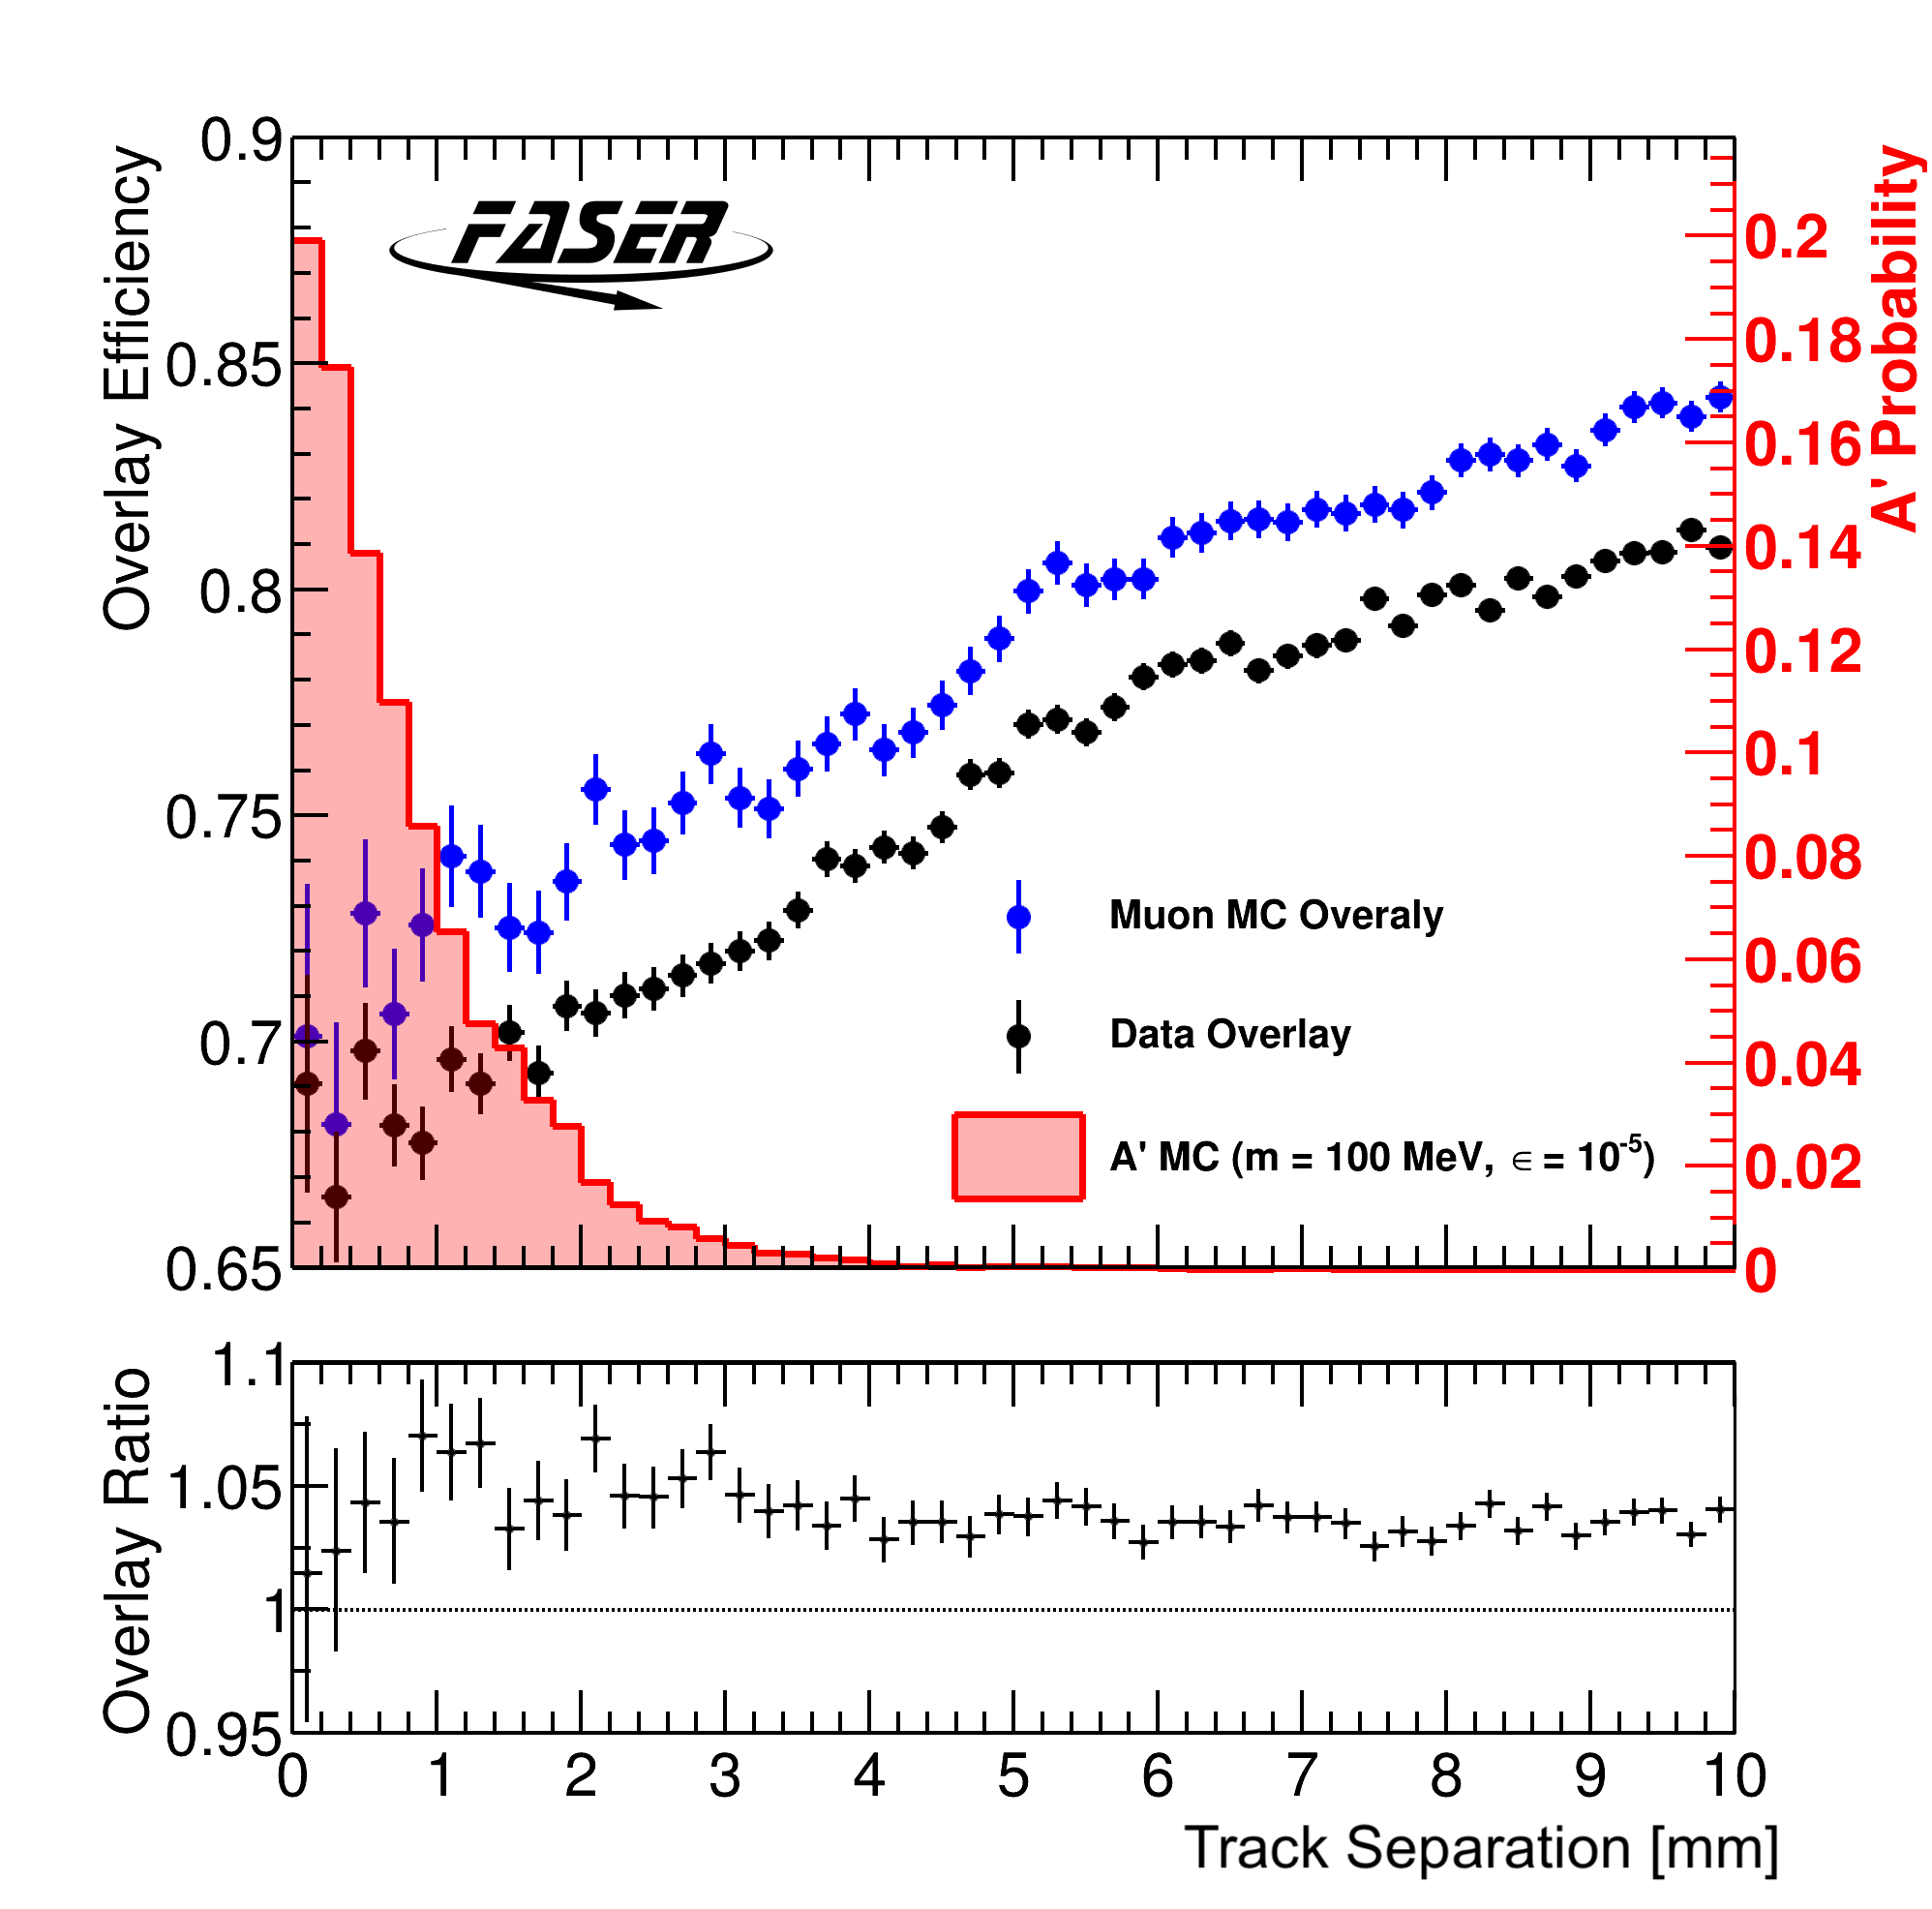
\includegraphics[width=0.8\textwidth]{assets/OverlayTracks.png}
                \caption{Overlay plot from Dark Photon Analysis}
            \end{figure}
        \end{column}
        \begin{column}{0.5 \textwidth}
            \begin{figure}
                \centering
                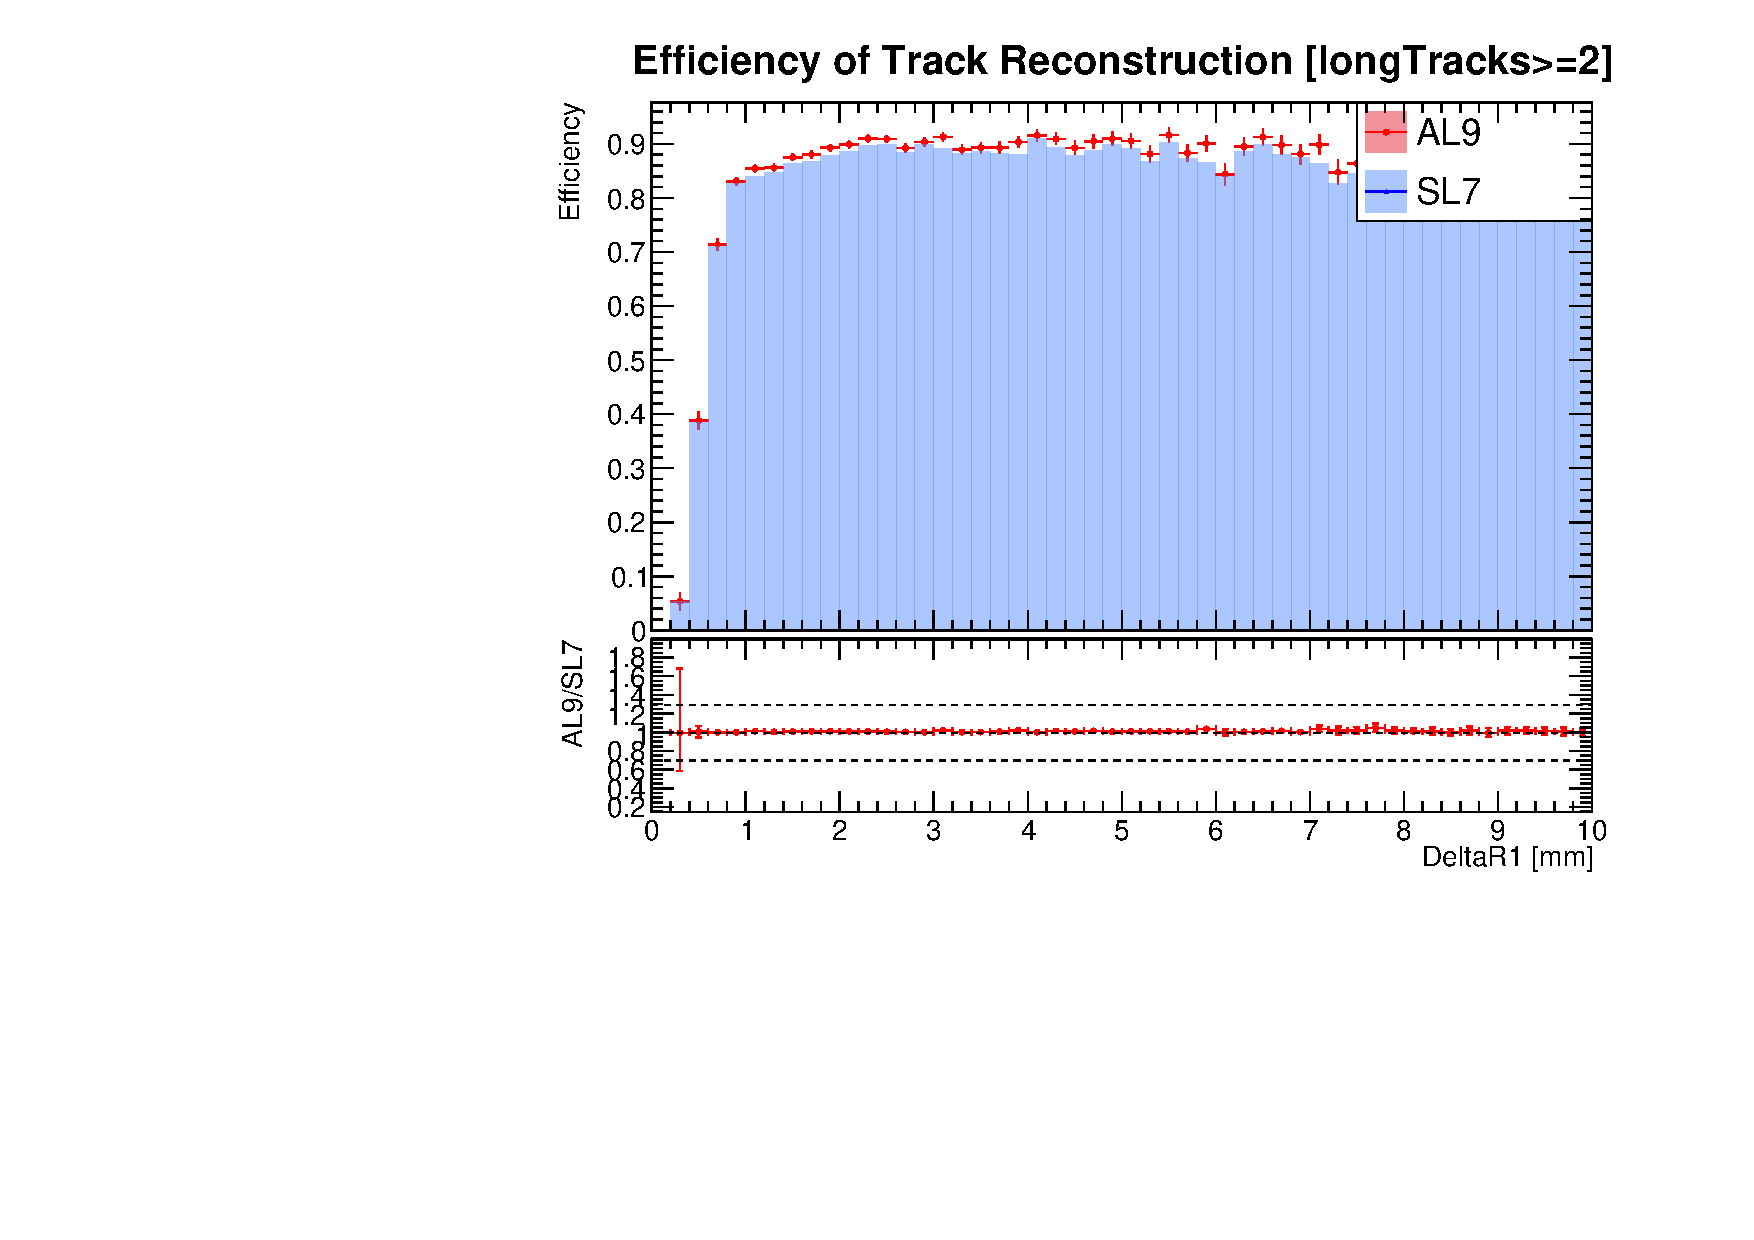
\includegraphics[width=1.1\textwidth]{assets/NEffi_greq2_DeltaR1.pdf}
                \caption{Track Efficiency ($\geq$2) as a function of distance between the tracks at the final station}
            \end{figure}
        \end{column}
    \end{columns}
    \begin{itemize}
        \item Not looking great for us \ldots 
        \item But atleast good agreement between ALMA9 and CENTOS7
        % \item Hopefully,
    \end{itemize}
\end{frame}